%% FEUP THESIS STYLE for LaTeX2e
%% how to use feupteses (English version)
%%
%% FEUP, JCL & JCF, 31 July 2012
%%
%% PLEASE send improvements to jlopes at fe.up.pt and to jcf at fe.up.pt
%%

%%========================================
%% Commands: pdflatex tese
%%           bibtex tese
%%           makeindex tese (only if creating an index)
%%           pdflatex tese
%% Alternative:
%%          latexmk -pdf tese.tex
%%========================================

\documentclass[11pt,a4paper,twoside,openright]{report}
% TODO: Open right

%% For iso-8859-1 (latin1), comment next line and uncomment the second line
\usepackage[utf8]{inputenc}
\usepackage{float}
%\usepackage[latin1]{inputenc}

%% English version

%% MIEIC options
%\usepackage[mieic]{feupteses}
\usepackage[mieic,juri]{feupteses}
%\usepackage[mieic,final]{feupteses}
%\usepackage[mieic,final,onpaper]{feupteses}

%% Additional options for feupteses.sty:
%% - onpaper: links are not shown (for paper versions)
%% - backrefs: include back references from bibliography to citation place

%% Include color package

%% Include source-code listings package


%% Uncomment to create an index (at the end of the document)
%\makeindex

%% Path to the figures directory
%% TIP: use folder ``figures'' to keep all your figures
\graphicspath{{figures/}}

%%----------------------------------------
%% TIP: if you want to define more macros, use an external file to keep them
%some macro definitions

% format
\newcommand{\class}[1]{{\normalfont\slshape #1\/}}

% entities
\newcommand{\Feup}{Faculdade de Engenharia da Universidade do Porto}

\newcommand{\svg}{\class{SVG}}
\newcommand{\scada}{\class{SCADA}}
\newcommand{\scadadms}{\class{SCADA/DMS}}

% color
\usepackage{color}
\definecolor{cloudwhite}{cmyk}{0,0,0,0.025}
\usepackage[dvipsnames]{xcolor}

% Code
\newcommand{\code}[1]{\path{#1}}

% Math
\usepackage{amsmath}
\newcommand{\pr}{\mbox{Pr}}
\newcommand{\gFunc}[1][d]{\displaystyle\prod_{j \in (d \cap obs_i)} g_j}

% Listings

\usepackage{listings}
\lstset{ %
 language=C,                        % choose the language of the code
 basicstyle=\footnotesize\ttfamily,
 keywordstyle=\bfseries,
 numbers=left,                      % where to put the line-numbers
 numberstyle=\scriptsize\texttt,    % the size of the fonts that are used for the line-numbers
 stepnumber=1,                      % the step between two line-numbers. If it's 1 each line will be numbered
 numbersep=8pt,                     % how far the line-numbers are from the code
 frame=tb,
 float=htb,
 aboveskip=8mm,
 belowskip=4mm,
 backgroundcolor=\color{cloudwhite},
 showspaces=false,                  % show spaces adding particular underscores
 showstringspaces=false,            % underline spaces within strings
 showtabs=false,                    % show tabs within strings adding particular underscores
 tabsize=2,                     % sets default tabsize to 2 spaces
 captionpos=b,                      % sets the caption-position to bottom
 breaklines=true,                   % sets automatic line breaking
 breakatwhitespace=false,           % sets if automatic breaks should only happen at whitespace
 escapeinside={\%*}{*)},            % if you want to add a comment within your code
 morekeywords={*,var,template,new}  % if you want to add more keywords to the set
}

\lstdefinestyle{npmlog}{
  moredelim=**[is][\color{gray}]{?}{?},
  moredelim=**[is][\color{ForestGreen}]{@}{@},
  moredelim=**[is][\color{purple}]{!}{!},
}

\lstdefinelanguage{Javascript}{
  keywords={break, case, catch, continue, debugger, default, delete, do, else, false, finally, for, function, if, in, instanceof, new, null, return, switch, this, throw, true, try, typeof, var, void, while, with},
  morecomment=[l]{//},
  morecomment=[s]{/*}{*/},
  morestring=[b]',
  morestring=[b]",
  ndkeywords={class, export, boolean, throw, implements, import, this},
  keywordstyle=\color{blue}\bfseries,
  ndkeywordstyle=\color{darkgray}\bfseries,
  identifierstyle=\color{black},
  commentstyle=\color{purple}\ttfamily,
  stringstyle=\color{red}\ttfamily,
  sensitive=true
}
%%----------------------------------------

%%========================================
%% Start of document
%%========================================
\begin{document}

%%----------------------------------------
%% Information about the work
%%----------------------------------------
\title{Software Repository Mining for Estimating Software Component Reliability}
\author{André Duarte}

%% Comment next line if not necessary for degree
% \degree{Programa Doutoral em Engenharia Informática}

%% Uncomment next line for date of submission
\thesisdate{June 24, 2016}

%% Comment next line copyright text if not used
% \copyrightnotice{Name of the Author, 2008}

\supervisor{Supervisor}{Rui Maranhão}
\supervisor{Second Supervisor}{Alexandre Perez}

%% Uncomment committee stuff in the final version if used
%\committeetext{Approved by \ldots:}
%\committeemember{President}{Name of the President}
%\committeemember{Referee}{Name of the Referee}
%\committeemember{Referee}{Name of the Referee}
%\signature

%% Specify cover logo (in folder ``figures'')
\logo{uporto-feup.pdf}

%% Uncomment next line for additional text below the author's name (front page)
%\additionalfronttext{Preparação da Dissertação}

%%----------------------------------------
%% Preliminary materials
%%----------------------------------------

% remove unnecessary \include{} commands
\begin{Prolog}
  \chapter*{Abstract}
%\addcontentsline{toc}{chapter}{Abstract}

TODO

\vspace*{10mm}\noindent

\textbf{Keyworks}: \emph{Software-fault Localization}, \emph{Software Repository Mining}, \emph{Machine Learning}, \emph{Classification}

\vspace*{5mm}\noindent

\textbf{Classificação}: \emph{Software and its engineering - Software creation and management - Software verification and validation; Computing methodologies - Machine Learning - Machine Learning Approaches}

\chapter*{Resumo}
%\addcontentsline{toc}{chapter}{Resumo}

Dada a crescente necessidade de identificar a localização dos erros no código fonte de \emph{software}, de forma a facilitar o trabalho dos programadores e a acelerar o processo de desenvolvimento, muitos avanços têm sido feitos na sua automação.

Existem três abordagens principais: \emph{Program-spectra based} (PSB), \emph{Model-based diagnosis} (MDB) e \emph{Program slicing}.

\emph{Barinel}, solução que integra tanto o PSB como o MDB, é, até hoje, com base na investigação feita, a que apresenta melhores resultados. Contudo, a ordenação de conjuntos de candidatos (componentes faltosos) não tem em conta a verdadeira qualidade do componente em causa, mas sim o conjunto de valores que maximizam a probabilidade do conjunto (\emph{Maximum Likehood Estimation} - MLE), devido à dificuldade da sua determinação.

Com esta tese pretende-se colmatar esta falha e contribuir para uma melhor ordenação dos conjuntos, classificando, com recurso a técnicas de Machine Learning como \emph{Naive Bayes}, \emph{Support Vector Machines} (SVM) ou \emph{Random Forests}, a qualidade e fiabilidade de cada componente, através das informações disponíveis no sistema de controlo de versões (\emph{Software Repository Mining}), neste caso \emph{Git}, como por exemplo: número de vezes que foi modificado, número de contribuidores, data de última alteração, nome de últimos contribuidores e tamanho das alterações.

A investigação já feita, revelou a existência de algumas soluções de análise preditiva de \emph{software}, como \emph{BugCache}, \emph{FixCache} e \emph{Change Classification}, capazes de identificar componentes com grande probabilidade de falhar e de classificar as revisões (\emph{commits}) como faltosas ou não, mas nenhuma soluciona o problema.

Este trabalho visa também a integração com o \emph{Crowbar} e a contribuição para a sua possível comercialização.

\vspace*{10mm}\noindent

\textbf{Palavras-chave}: \emph{Software-fault Localization}, \emph{Software Repository Mining}, \emph{Machine Learning}, \emph{Classification}

\vspace*{5mm}\noindent

\textbf{Classificação}: \emph{Software and its engineering - Software creation and management - Software verification and validation; Computing methodologies - Machine Learning - Machine Learning Approaches} % the abstract
  \chapter*{Agradecimentos}
%\addcontentsline{toc}{chapter}{Agradecimentos}

Aliquam id dui. Nulla facilisi. Nullam ligula nunc, viverra a, iaculis
at, faucibus quis, sapien. Cum sociis natoque penatibus et magnis dis
parturient montes, nascetur ridiculus mus. Curabitur magna ligula,
ornare luctus, aliquam non, aliquet at, tortor. Donec iaculis nulla
sed eros. Sed felis. Nam lobortis libero. Pellentesque
odio. Suspendisse potenti. Morbi imperdiet rhoncus magna. Morbi
vestibulum interdum turpis. Pellentesque varius. Morbi nulla urna,
euismod in, molestie ac, placerat in, orci. 

Ut convallis. Suspendisse luctus pharetra sem. Sed sit amet mi in diam
luctus suscipit. Nulla facilisi. Integer commodo, turpis et semper
auctor, nisl ligula vestibulum erat, sed tempor lacus nibh at
turpis. Quisque vestibulum pulvinar justo. Class aptent taciti
sociosqu ad litora torquent per conubia nostra, per inceptos
himenaeos. Nam sed tellus vel tortor hendrerit pulvinar. Phasellus
eleifend, augue at mattis tincidunt, lorem lorem sodales arcu, id
volutpat risus est id neque. Phasellus egestas ante. Nam porttitor
justo sit amet urna. Suspendisse ligula nunc, mollis ac, elementum
non, venenatis ut, mauris. Mauris augue risus, tempus scelerisque,
rutrum quis, hendrerit at, nunc. Nulla posuere porta orci. Nulla dui. 

Fusce gravida placerat sem. Aenean ipsum diam, pharetra vitae, ornare
et, semper sit amet, nibh. Nam id tellus. Etiam ultrices. Praesent
gravida. Aliquam nec sapien. Morbi sagittis vulputate dolor. Donec
sapien lorem, laoreet egestas, pellentesque euismod, porta at,
sapien. Integer vitae lacus id dui convallis blandit. Mauris non
sem. Integer in velit eget lorem scelerisque vehicula. Etiam tincidunt
turpis ac nunc. Pellentesque a justo. Mauris faucibus quam id
eros. Cras pharetra. Fusce rutrum vulputate lorem. Cras pretium magna
in nisl. Integer ornare dui non pede. 

\vspace{10mm}
\flushleft{O Nome do Autor}
  % the acknowledgments
  \cleardoublepage
\thispagestyle{plain}

\vspace*{8cm}

\begin{flushright}
   \textsl{``You should be glad that bridge fell down. \\
           I was planning to build thirteen more to that same design''} \\
\vspace*{1.5cm}
           Isambard Kingdom Brunel
\end{flushright}
    % initial quotation if desired
  \cleardoublepage
  \pdfbookmark[0]{Table of Contents}{contents}
  \tableofcontents
  \cleardoublepage
  \pdfbookmark[0]{List of Figures}{figures}
  \listoffigures
  \cleardoublepage
  \pdfbookmark[0]{List of Tables}{tables}
  \listoftables
  \chapter*{Abreviaturas e Símbolos}
%\addcontentsline{toc}{chapter}{Abbreviations}
\chaptermark{ABREVIATURAS E SÍMBOLOS}

\begin{flushleft}
\begin{tabular}{l p{0.8\linewidth}}
MSR 	 & Mining Software Repositories\\

\end{tabular}
\end{flushleft}

  % the list of abbreviations used
\end{Prolog}

%%----------------------------------------
%% Body
%%----------------------------------------
\StartBody

%% TIP: use a separate file for each chapter
%!TEX root = ../thesis.tex
\chapter{Introdução} \label{chap:intro}

\section*{}

Pretende-se com este capítulo enquadrar o tema, explicar as motivações e descrever sucintamente a estrutura deste documento.

\section{Contexto/Enquadramento} \label{sec:context}

Com o elevado crescimento da indústria de desenvolvimento de software,
torna-se cada vez mais importante a existência de ferramentas que auxiliem
os programadores a desenvolvê-lo mais eficientemente.

Estima-se que a economia dos Estados Unidos perca entre 60 mil milhões de dólares por ano em custos associados ao desenvolvimento e distribuição de correções para defeitos de \emph{software} e na sua reinstalação \cite{Zhivich2009}. Pelo que, podemos afirmar que as ferramentas de localização das falhas de \emph{software} (\emph{Software Fault Localization}), ajudando a reduzir o tempo investido nesta tarefa, poderão ter um impacto significativo na economia.
Nesta área os avanços são consideráveis. \emph{Ochiai}, \emph{Tarantula}, \emph{Bayes-A} e \emph{Barinel} são apenas algumas das soluções existentes, sendo o algoritmo \emph{Barinel} aquele que apresenta melhores resultados. \cite{Abreu2009}
Apesar dos bons resultados apresentados pelo \emph{Barinel}, este poderá apresentar resultados ainda mais rigorosos se tivermos informações relativas ao projeto, como a probabilidade média de erro ou a probabilidade de dado componente, que o constitui, ter defeitos.

Ferramentas de controlo de versões, como o \emph{Git}, uma vez que mantêm todo o histórico do projeto e informações relacionadas com as diversas alterações (p.e. conteúdo, data e autores), em conjunto com técnicas de \emph{Machine Learning}, poderão ser a chave para a melhoria deste algoritmo.

\section{Motivação e Objetivos} \label{sec:goals}

Tendo em conta as possibilidades que a extração de dados de repositórios de controlo de versões e o \emph{Machine Learning} nos dão, pretende-se com esta dissertação:
%
\begin{itemize}
\item Optimizar a ordenação de resultados candidatos do algoritmo Barinel.
\item Ter a capacidade de prever a probabilidade de defeito de cada um dos componentes de um dado projecto de \emph{software}, que use o \emph{Git} para controlo total de versões, com uma precisão útil.
\end{itemize}

\section{Estrutura} \label{sec:struct}

% TODO: CHANGE

% Para além da introdução, esta dissertação contém mais 4 capítulos.
% No capítulo~\ref{chap:sota}, é descrito o estado da arte e são apresentados trabalhos relacionados com \emph{fault localization software}, \emph{software repository mining} e ainda algumas abordagens à previsão de defeitos. No capítulo~\ref{chap:chap3}, expõe-se a perspetiva de solução e contrasta-se com as possíveis dificuldades que poderão ser encontradas durante a sua realização, apresentando no capítulo seguinte~\ref{chap:chap4} a forma como esta deve ser validada. Por último, o capítulo~\ref{chap:concl} conclui o relatório e explicita o plano de trabalhos, na forma de um gráfico de \emph{Gantt}.

%!TEX root = ../thesis.tex
\chapter{State of the art} \label{chap:sota}

\section*{}

Neste capítulo é feita uma revisão bibliográfica e descrito o estado da arte do \emph{software} de localização de falhas, como o \emph{Barinel}, das diferentes abordagens de predição de defeitos e ainda de \emph{Software Repository Mining}.

%!TEX root = ../thesis.tex
\section{Fault Localization Software}

Fault Localization Software helps to automatically locate code that generates faults when it is executed, reducing the costs associated with finding it, which would have to be done manually by the developer.  There are three main types of approach: \emph{Program Slicing}, \emph{Spectrum-based diagnosis} and \emph{Model-based diagnosis}. The \emph{Spectrum-based diagnosis} approaches will have a more detailed analysis due to their greater relevance to this work.

% 
% ==========
% Program Slicing
% ==========
%

\subsection{\emph{Program Slicing}}

Introduced by Mark Weiser in 1981 \cite{Weiser1981, Weiser1982}, this method starts its analysis from the fault and, by way of the program's data and control flow, tries to find where the problem originates. 

By removing all statements that won't affect the data set or program flow, this method determines a section of code (slice) corresponding to all statements that may be the root of the problem and must be inspected. \cite{Perez2004}. By reducing the amount of statements that require inspection, the time needed to fix an error is also reduced.

Usually, a static analysis of the program will result in a huge section of code, so there are other, dynamic, methods that will considerably reduce its size, such as \emph{program dice} or \emph{dynamic program slicing} \cite{Perez2004}.

% 
% ==========
% Spectrum-based diagnosis
% ==========
%

\subsection{\emph{Spectrum-based diagnosis}}

\emph{Spectrum-based Fault Localization} (SFL) is a probability-based fault detection method that will estimate each software component's probability of containing faults by analyzing execution-related information, whether that execution is successful or not \cite{Abreu2007}. This method is able to generate good results when the project contains a big amount of test cases and can be executed swiftly, being able to scale well to big projects \cite{Mayer2008}.

This method generates a matrix based of data saved during the execution (\emph{program spectrum} \cite{Reps1997}), connecting each test case ran with the components executed and the result, successful or unsuccessful, of that test.

\begin{table}[H]
  \centering
  \begin{tabular}{c|ccc|c} 
    & \multicolumn{3}{c|}{\textit{obs}} &  \\
    & $c_1$ & $c_2$ & $c_3$ & e \\ 
    \hline
    $t_1$ & 1 & 1 & 0 & 1 \\
    $t_2$ & 0 & 1 & 1 & 1 \\
    $t_3$ & 1 & 0 & 0 & 1 \\
    $t_4$ & 1 & 0 & 1 & 0 \\
  \end{tabular}
  \caption{\emph{Hit-spectra matrix}}
  \label{tab:hit-spectra}
\end{table}

With this matrix, also called \emph{hit-spectra matrix}, a \emph{similarity coefficient} is calculated for each of the components \cite{Abreu2009}, showing how likely it is that a component may have a fault. The way this coefficient is calculated is different, depending on the algorithm used. For example, \emph{Pinpoint} \cite{Chen2002}, \emph{Tarantula} \cite{Jones2005} and \emph{Ochiai} \cite{Abreu2007}, each, respectively, calculate the coefficient as follows
%
\begin{equation}
  s_J(j) = \frac {a_{11}(j)} {a_{11}(j) + a_{01}(j) + a_{10}(j)}
\end{equation}
%
\begin{equation}
  s_T(j) = \frac  { \frac {a_{11}(j)} {a_{11}(j) + a_{01}(j)} } 
          { \frac{a_{11}(j)}{a_{11}(j) + a_{01}(j)} + \frac{a_{10}(j)}{a_{10}(j) + a_{00}(j)}}
\end{equation}
%
\begin{equation}
  s_O(j) = \frac  {a_{11}(j)} 
          {\sqrt{(a_{11}(j) + a_{01}(j)) * (a_{11}(j) + a_{10}(j))}}
\end{equation}


% 
% ==========
% Model-based diagnosis
% ==========
%

\subsection{\emph{Model-based diagnosis}}

The basis of \emph{Model-based diagnosis} is comparing the model, i.e. the description of the system's behavior, with the actually observed behavior \cite{Mayer2008}. The difference between the two is then used to identify components that may explain errors occurred. This actually requires a formal description of the system,  which makes the task harder \cite{Perez2004}.

In order to facilitate using this method, the model is usually inferred by using the software itself, specifically, by using the test cases defined in it \cite{Perez2004}.

Although this method generates high-reliability results, the computational effort required to create a model for a big program will prevent it to be used in real projects most of the times \cite{Mayer2008}.

% 
% ==========
% Barinel
% ==========
%

\subsection{Barinel}

Barinel is an algorithm inspired by the two methods previously described, \emph{program-spectra based} and \emph{model-based diagnosis}, thus being able to generate better results than the other approaches, albeit with a slightly higher cost \cite{Abreu2009}.

This algorithm starts by analyzing a \emph{hit-spectra matrix}, representing a connection between the executed tests, the executed components, and their final result.

\begin{table}[H]
  \centering
  \begin{tabular}{c|ccc|c} 
    & \multicolumn{3}{c|}{\textit{obs}} &  \\
    & $c_1$ & $c_2$ & $c_3$ & e \\ 
    \hline
    $t_1$ & 1 & 1 & 0 & 1 \\
    $t_2$ & 0 & 1 & 1 & 1 \\
    $t_3$ & 1 & 0 & 0 & 1 \\
    $t_4$ & 1 & 0 & 1 & 0 \\
  \end{tabular}
  \caption{\emph{Hit-spectra matrix}}
  \label{tab:hit-spectra}
\end{table}


In the table \ref{tab:hit-spectra}, we have identified 3 distinct components ($c_1$, $c_2$ e $c_3$), 4 executed tests ($t_1$, $t_2$, $t_3$ e $t_4$) and the result of their execution ($e$). A value of 1 in any of the observation columns (\emph{obs}) shows that the specific component has been executed in that test, while a value of 0 shows the opposite, the component has not been executed in that test. For the column $e$, a value of 1 indicates that the corresponding test has failed. 
For example, the test $t_4$ has executed the components $c_1$ and $c_3$ and completed successfully.


% 
% Generating candidates
%

\subsubsection{Generating candidates} 

Using this matrix, a list of candidate sets ($d$) is generated. This list is reduced to the lowest possible amount of candidates, as they encompass all other candidates and allow a reduction of the search space. This problem, entitled \emph{minimal hitting set} (MHS), is itself an \emph{NP-hard} problem, which means specific heuristics had to be created \cite{RuiAbreu, Cardoso2013}. The algorithm used by Barinel to resolve this problem is \emph{Staccato}.

In this case, only two candidates would be generated:

\begin{itemize}
\item $d_1 = \{c_1, c_2\}$ 
\item $d_2 = \{c_1, c_3\}$ 
\end{itemize}

% 
% Candidate sorting
%

\subsubsection{Candidate sorting} 

For each candidate $d$, a probability is calculated using a \emph{Naïve Bayes} model:
%
\begin{equation}
  \pr(d\mid obs,e) =  \pr(d) \cdot \prod_{i}\frac{\pr(obs_i, e_i \mid d)}{\pr(obs_i)}
\end{equation}


$Pr(obs_i)$ is just a normalized term, identical for every candidate and not used for sorting.

Being $p_j$ the \emph{a priori} probability of component $c_j$ causing a fault, also called \emph{prior}, we can define $Pr(d)$, the probability of the candidate being responsible for the error, without taking into account additional evidence, such as
%
\begin{equation}
  \pr(d) = \prod_{j \in d} p_j \cdot \prod_{j \notin d} (1 - p_j)
\end{equation}


Being $g_j$ (\emph{component goodness}) the probability of component $c_j$ executing correctly if $c_j$ is part of the faulty components set, we have
% 
\begin{equation}
  \pr(obs_i, e_i \mid  d) = 
  \begin{cases}
    \gFunc    & \textrm{if} e_i = 0 \\
  1 - \gFunc  & \textrm{otherwise}
  \end{cases}
\end{equation}

Taking our example into account
%
\begin{equation}
    \pr(d_1 \mid obs,e) =
    \overbrace{\bigg(\frac{1}{1000} \cdot \frac{1}{1000} \cdot \bigg(1 - \frac{1}{1000}\bigg)\bigg)}^{\pr(d)}
    \times
    \overbrace{
      \underbrace{(1-g_1 \cdot g_2)}_{t_1}
      \times
      \underbrace{(1-g_2)}_{t_2}
      \times
      \underbrace{(1-g_1)}_{t_3}
      \times
      \underbrace{g_1}_{t_4}
    }^{\pr(obs,e \mid d)}
\end{equation}
%
\begin{equation}
    \pr(d_2 \mid obs,e) =
    \overbrace{\bigg(\frac{1}{1000} \cdot \frac{1}{1000} \cdot \bigg(1 - \frac{1}{1000}\bigg)\bigg)}^{\pr(d)}
    \times
    \overbrace{
      \underbrace{(1-g_1)}_{t_1}
      \times
      \underbrace{(1-g_3)}_{t_2}
      \times
      \underbrace{(1-g_1)}_{t_3}
      \times
      \underbrace{g_1 \cdot g_3}_{t_4}
    }^{\pr(obs,e \mid d)}
\end{equation}


In cases where there are unknown $g_j$ values, the value of $Pr(obs, e | d)$ is maximized using the \emph{Maximum Likelihood Estimation} (MLE) algorithm.

In this case, all of $g_j$ values are unknown. Applying the MLE algorithm to both functions and calculating the final result gives us:
%
\begin{itemize}
\item $Pr(d_1, obs, e) = 1.9 \times 10^{-9}$\ \ ($g_1 = 0.47$ e $g_2 = 0.19$)
\item $Pr(d_2, obs, e) = 4.0 \times 10^{-10}$ ($g_1 = 0.41$ e $g_3 = 0.50$)
\end{itemize}


% 
% ==========
% Crowbar
% ==========
%
\subsubsection{\emph{Crowbar}}

\emph{Crowbar}\footnote{ \url{http://crowbar.io}}, formerly known as GZoltar\footnote{ \url{http://www.gzoltar.com/}}, is the tool used to materialize the Barinel algorithm and that allows the analysis of \emph{Java} projects \cite{Campos2012}.

By using code injection and running \emph{JUnit} tests, \emph{Crowbar} is able to identify executed components and connect them to unsuccessful tests.

There are different ways to present the results, the main one being the \emph{Sunburst} visualization, shown in Figure~\ref{fig:crowbar-sunburst}, where each ring represents a different granularity level, from the project to a line of code \cite{Gouveia2013}.
%
\begin{figure}[H]
  \begin{center}
    \leavevmode
    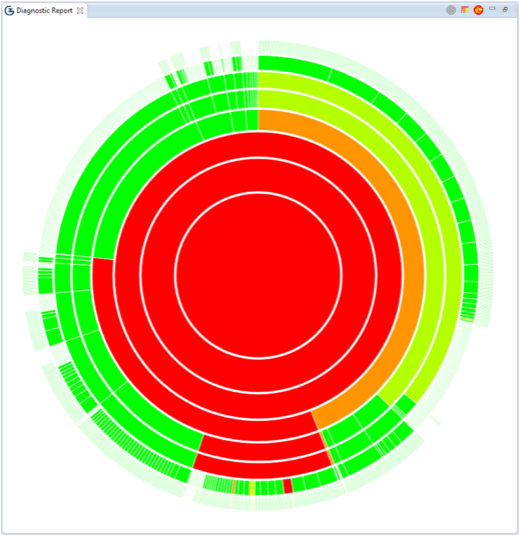
\includegraphics[width=0.5\textwidth]{barinel1.png}
    \caption{Sunburst visualization on Crowbar}
    \label{fig:crowbar-sunburst}
  \end{center}
\end{figure}

In addition to that information, this tool also shows us the component list sorted by fault likelihood.
%!TEX root = ../thesis.tex
\section{\emph{Software Repository Mining}}

\emph{Software Repository Mining} encompasses all \emph{software} which is able to extract data from repositories, such as \emph{Git} or \emph{SVN}.

\subsection{Corrections and defects identification}

While extracting information from code repositories, such as \emph{Git}, it is important to identify the types of changes that were made. A text description associated with the change is of the utmost importance for this identification, allowing it to be made with a high degree of precision, depending on the project \cite{Mockus2000}.

It is estimated that between 34 and 46\% of all changes are corrections and that they represent between 18 and 27\% of all added and removed lines of code \cite{Mockus2000}. There were also some patterns found relating code corrections with their size and with the day of the week in which they were executed \cite{Sliwerski2005}.

After this identification, it is possible to find out which changes have introduced the errors by using the \emph{SZZ} algorithm \cite{Sliwerski2005}. This algorithm analyzes the code and uses its history to correctly locate which \emph{commit} has introduced the defect, ignoring changes that only inserted comments, for example.

\subsection{Tools}

There are several tools to facilitate this process. Let us highlight two of them.

\subsubsection{\emph{libgit2}}

Libgit2\footnote{\url{https://libgit2.github.com/}} is a multi-platform library, without dependences, allowing a direct and native performance interaction with the \emph{Git} repository.

This library can be used with any language supporting \emph{C} bindings, so there are dozens of implementations using languages like \emph{Python}\footnote{pygit2 - \url{http://www.pygit2.org/}}, \emph{Javascript}\footnote{nodegit - \url{https://github.com/nodegit/nodegit}} and \emph{Java}\footnote{Jagged - \url{https://github.com/ethomson/jagged}}.

\subsubsection{\emph{GHTorrent}}

GHTorrent\footnote{\url{http://ghtorrent.org/}} is a project with the objective of creating a scalable and easily queriable (even \emph{offline}) database, which replicates the information obtained through the GitHub\footnote{\url{http://developer.github.com/}} REST API.

This tool works in a distributed way and monitors the GitHub API through the page \url{https://api.github.com/events}. Each event triggers an information and content extraction to a \emph{MongoDB} database and a different \emph{MySQL} database \cite{Gousios2012}.
%!TEX root = ../thesis.tex
\section{Approaches to defect prediction}

We have already explored some approaches to code quality prediction. In this chapter we will highlight some methods, like \emph{BugCache}, \emph{FixCache} and \emph{Buggy Change Classification}, which are included in the type of approach we want to follow (\emph{change log}) and that allow us, together with other methods, to optimize defect localization.

\subsection{\emph{BugCache/FixCache}}

Based on the assumption that faults never occur isolated, and therefore where there's a defect others can also exist, \emph{BugCache} creates a list of components which have a high probability of containing defects, based on an analysis of the complete changes history of the project.

This algorithm stands out due to its precision, managing a 73 to 95\% accuracy when used with file-level granularity, being the best to date \cite{kim2006automatic}.

Defects are identified by order of occurrence and added to the list. When that list reaches its maximum size, components start to be removed according to the chosen substitution method. There are several methods using different metrics, such as \emph{Least Recent Used - LRU}, number of recent defects and number of recent changes \cite{kim2006automatic}.

With this algorithm, we can conclude \cite{kim2006automatic}:
%
\begin{itemize}
	\item If a defect has been introduced, there is a tendency to soon introduce additional new defects (\emph{temporal locality})
	\item If a component was added or changed recently, it has a higher probability of defect (\emph{changed-entity locality}, \emph{new-entity locality})
	\item If a component has introduced an error, the components most directly connected to that one will also introduce errors in the future (\emph{spatial locality})
\end{itemize}

The difference between \emph{BugCache} and \emph{FixCache} is the time at which each one updates the list. The former updates the list when a defect is introduced, while the latter only updates when the error is fixed. Due to this difference, implementing \emph{FixCache} is easier.

\subsection{\emph{Buggy Change Classification}}

\emph{Change Classification} has a notably different approach and a very distinct objective too. \emph{Change Classification}, resorting to \emph{Machine Learning} methods and available information about previous errors, is able to predict if a change has introduced a new defect. This prediction has a high accuracy of 78\% \cite{Whitehead2008}.

In a first phase, all changes up to that moment are either classified as \emph{buggy} or \emph{clean}. After classifying them and extracting data for each one, a model is created by \"training\" a classification algorithm.

The types of data used are divided in seven groups: complexity metrics, added code, removed code, file and folder names, new code and meta-data \cite{Whitehead2008}.

Both \emph{Support Vector Machine} (SVM) and \emph{Naive Bayes} were used in the study, with the SVM-based classifier being the one with better results \cite{Whitehead2008}.

\subsection{Data-Augmented Software Diagnosis} \label{subsec:elmishali}

A different approach that also aims to help predict the location of software faults is Data-Augmented Software Diagnosis \cite{Elmishali}.

Model-based and spectrum-based approaches are able to identify faulty components with high precision and recall, but there is still room for improvement and since most projects use some kind of Version Control Software (VCS), there is a big amount of information that is not used. This opportunity is the foundation of the approach.

Barinel assumes that the defect probability, known as the prior, of every component is uniform, $0.001$. However, this approach proved it is possible to optimize Barinel results for Java projects by leveraging information about the project and supervised machine learning algorithms to predict the real component's defect probability.

First, healthy and faulty components are identified across the entire project's history according to Bug Trackers. For each component, a list of features, which is not specified, is extracted. The list is composed of traditional and object-oriented software complexity metrics, such as number of lines of code and cohesion, and values extracted from the software change history, like lines added or removed in last version and age of the file.

With the help of a supervised machine learning algorithm (either Random Forest, J48 or Naive Bayes) a model is created and used to classify each component in the project as healthy or faulty. The confidence that a component is faulty is then used as prior.

Experimental results revealed an increment both on precision and recall, see Figure \ref{fig:elmishali}. However, the solution was tested just on one project.
%
\begin{figure}%
    \centering
    \subfloat[Precision]{{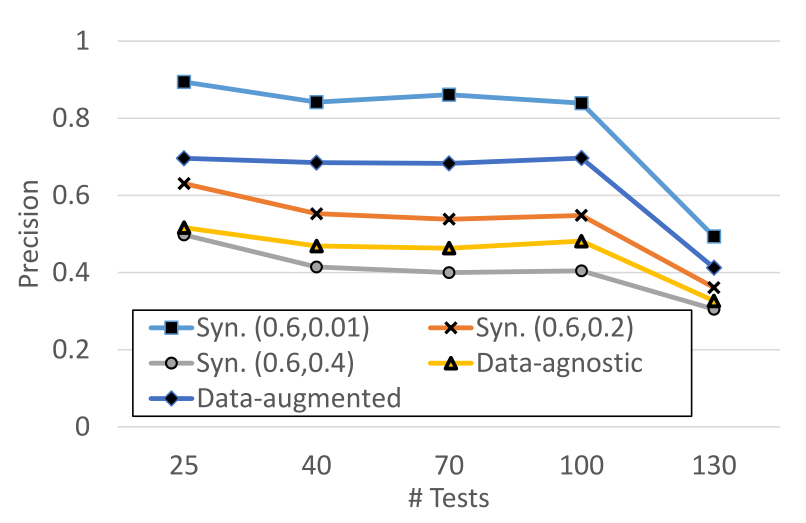
\includegraphics[width=0.4\textwidth]{elmishali-precision} }}%
    \qquad
    \subfloat[Recall]{{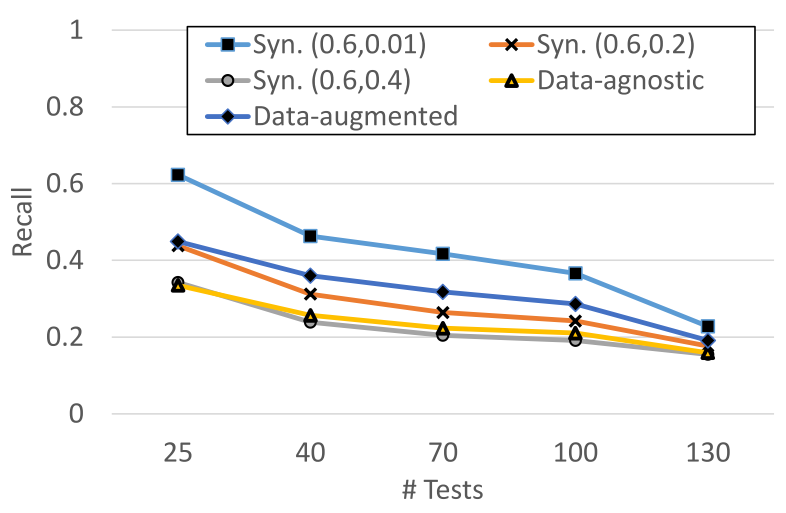
\includegraphics[width=0.4\textwidth]{elmishali-recall} }}%
    \caption{Diagnosis accuracy as a function of \# tests given to the diagnoser. \cite{Elmishali}}%
    \label{fig:elmishali}%
\end{figure}

\subsection{Time-weighted Risk}

Time-weighted risk is a formula developed at Google that helps in estimating component's reliability \cite{Lewis}. 
%
\begin{equation}
  \sum_{i=0}^{n}  \frac {1} {1 + e^{(-12 \cdot t_i) + W}}
\end{equation}

Where $i$ is a fixing commit, $t$ is the normalized change timestamp, from 0 to 1. If the change is at the start of the repository, the normalized timestamp will be 0. If instead the change is the last change made, the normalized timestamp will be 1. $W$ defines the weight of the decay, shifting the scoring curve along the x-axis.

The time-weighted curve produced by $\frac {1} {1 + e^{(-12 \cdot t_i) + W}}$ is the following:
%
\begin{figure}[H]
  \begin{center}
    \leavevmode
    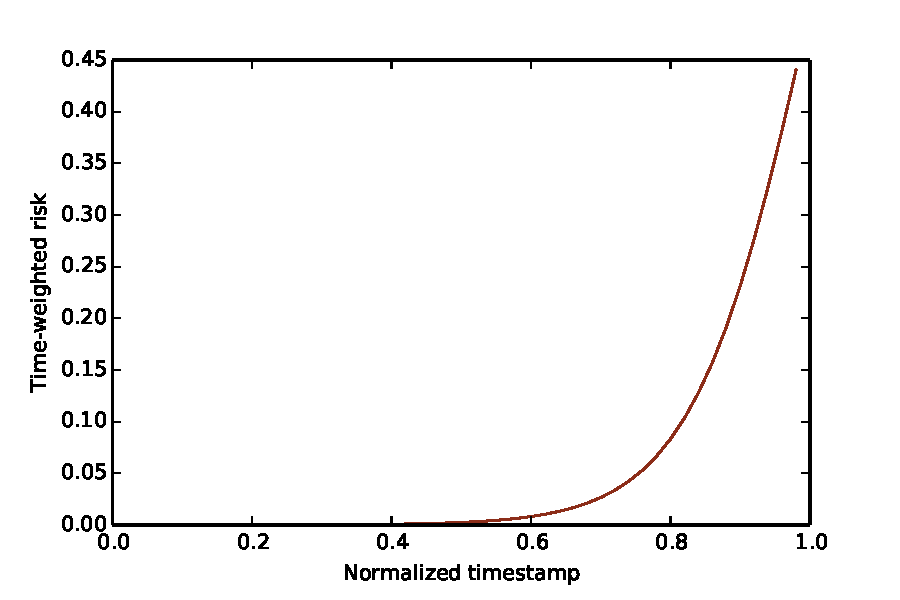
\includegraphics[width=0.5\textwidth]{twr.pdf}
    \caption{Time-weighted risk as function of the normalized timestamp of a given commit}
    \label{fig:crowbar-sunburst}
  \end{center}
\end{figure}

\todo{Talk about the Amir Elmishali's paper}

\todo{Add Background about Machine Learning?}
%!TEX root = ../thesis.tex
\chapter{Estimating Defect Probabilities} \label{chap:estimating-dp}

\section*{}

In order to estimate the defect probability of each software component we developed a data mining application, agnostic to the project's language. 
It automatically extracts data from the current state and about older defects from a \emph{Git} repository, creates a model and predicts the probability. The project is written in Javascript (Node.js) and Python 3 and heavily uses \emph{node-git}
and \emph{scikit-learn}.

In this chapter, we will explain the concept behind it, approach the process used in each of the steps and will explain how to install and use this application.

\section{Concept}

Some patterns are easily recognizable when trying to identify faulty components on a software project and this information could be helpful for software such as Barinel. 

We might say, for example that having a high number of recent changes or having been changed by a given junior developer new to the project probably increases the chances of a file having an error, due to past experiences. So, deep down we are just assuming that the knowledge of the meta-data of old faulty components may allow us to predict which components are more probable to be faulty, now.

Based on that assumption, the application, for a given repository state, extracts meta-data knowledge from past commits with faulty components, the parent commits of a fix. For each of these commits, all of components are analyzed and labeled as faulty or clean, if it was or not changed on the fix, respectively.
%
% CHOURIÇO:
%
%\begin{figure}[H]
%  \begin{center}
%    \leavevmode
%    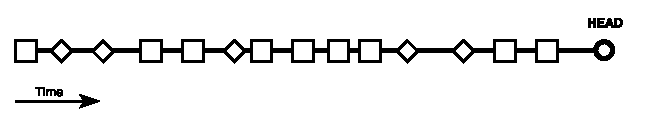
\includegraphics[width=0.7\textwidth]{commits.pdf}
%    \caption{Example representation of commits history, with fix commits illustrated in a diamond shape}
%    \label{fig:commits}
%  \end{center}
%\end{figure}

Since the application should be able to predict the defect probability for any given software project that uses \emph{Git}, static analysis is not used. 
The only information that is used is information directly related to the file changes, authors, number of lines or bytes.

Along with the extraction of the meta-data information from the past faulty states, it must also extract the meta-data of the given repository state. The data from the first extraction must be used to create a machine learning model, that should be able to predict the defect probability of each component presents in the current state of the project.
%
\begin{figure}[ht]
  \begin{center}
    \leavevmode
    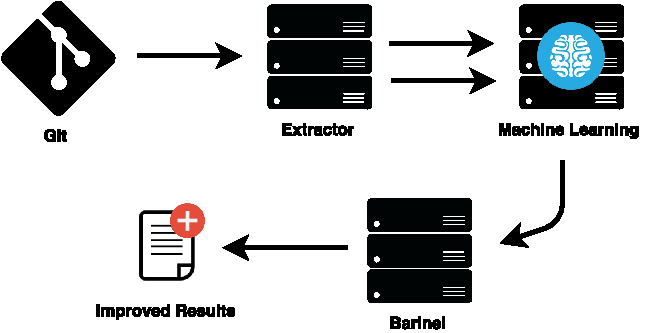
\includegraphics[width=0.7\textwidth]{concept.pdf}
    \caption{Representation of data flow}
    \label{fig:concept}
  \end{center}
\end{figure}

This concept differs from Data-Augmented Software Diagnosis (Subsection \label{subsec:elmishali}) by being language agnostic, requiring a different set of features mostly focused on number of changes, categorized by type and authors, and weighted according to size and date. It also differs by not requiring that the project uses a bug tracking software and also, as explained in the following section. 

\section{Install}

The application relies on \emph{Redis}, \emph{Git}, \emph{Node.js} and \emph{Python 3} and requires some dependencies such as \emph{SciPy}, \emph{scikit-learn}, \emph{numpy}.

\begin{lstlisting}
  $ git clone --depth 1 https://github.com/atduarte/master-thesis.git
  $ cd master-thesis/app
  $ npm install --prod
\end{lstlisting}

\section{Usage}

Having all the required dependencies installed, the usage is very straight-forward.
In order to automatically execute all the steps (extraction, data preparation, modeling and prediction) the following command should be used
by replacing "\code{{project-name}}" and "\code{{repository-path}}" respectively with
the chosen project name and the path to the folder containing the repository we want to analyze:

\begin{lstlisting}
  $ node index.js all {project-name} {repository-path}
\end{lstlisting}

It is possible to specify a different classification label (e.g. "\code{--classification-label=_mostChanged}", default is "\code{_mostChanged25}"), 
a different number of estimators used when modeling (e.g. "\code{--estimators=100}", default is 5) or even
to define the level of logging by appending, for example, "\code{--log-level=verbose}". The existing levels available, from higher to lower priority, are
"\code{error}", "\code{warn}", "\code{info}", "\code{verbose}" and "\code{silly}". The default log level is "\code{info}".

\begin{lstlisting}[style=npmlog]
  ?$  node index.js all math ../../tests/Math001?
  @info@ !extract/extract! Raw Extraction started
  @info@ !extract/extract! 499 fix commits found
  @info@ !prepareJson/prepare! JSON Preparation started
  @info@ !prepareJson/prepare! Will prepare 639 files
  @info@ !results/prepare! CSV Preparation started
  @info@ !results/prepare! Got 552 files
  @info@ !results/prepare! Got 203 columns
  @info@ !results/ml! Modeling
\end{lstlisting}

Some extra configurations are also available by creating a project configuration file, in the folder "\code{project-config/}", with the same name as the \code{project-name} plus ".js".
It allows to change the \emph{regex} used to identify the fix commits, to define a file filter and to define an email normalizer, in order to improve the quality of the extracted data .

\begin{lstlisting}[language=Javascript]
  'use strict';

  module.exports = {
      fileFilter: (filename) => {
          filename = filename.toLowerCase();

          return filename.endsWith('.java') // Is Java
              && !filename.startsWith('src/test'); // Aren't tests
      },
  };
\end{lstlisting}

Before terminating, the application will create a file ("\code{prediction.e500._mostChanged25.csv}", by default) in the repository folder containing the predicted defect probability for each source code file.

\begin{lstlisting}
  ...
  src/main/java/org/joda/time/Chronology.java,0.0
  src/main/java/org/joda/time/DateMidnight.java,0.21
  src/main/java/org/joda/time/DateTime.java,0.484
  src/main/java/org/joda/time/DateTimeComparator.java,0.0
  src/main/java/org/joda/time/DateTimeConstants.java,0.0
  src/main/java/org/joda/time/DateTimeField.java,0.006
  src/main/java/org/joda/time/DateTimeFieldType.java,0.002
  src/main/java/org/joda/time/DateTimeUtils.java,0.966
  src/main/java/org/joda/time/DateTimeZone.java,0.414
  src/main/java/org/joda/time/Days.java,0.0
  ...
\end{lstlisting}

In order to be able to execute only some step of the process, there is the possibility of executing only one operation. The available commands are:
%
\begin{itemize}
\item "\code{raw}" - Extracts data from \emph{Git} and saves it to "\code{out/{project-name}/raw}"
\item "\code{json}" - Processes the raw data and converts it to a new JSON structure. Results are saved to "\code{out/{project-name}/json}"
\item "\code{results}" - Creates the CSV files for training and prediction data, based on the JSON files, creates the model and predicts the defect probability.
Final result is saved at "\code{{repository-path}/prediction.csv}".
\end{itemize}

\section{Process}

As stated before the process is divided in extraction, data preparation, modeling and prediction steps. We will now dive deep into each.

\subsection{Extraction}

The first objective is to get the list of commits to analyze: the HEAD commit and all the fix commits that preceded it. 
So, first, the \emph{HEAD} commit is identified. The application then walks recursively through each parent commit or commits and,
if it is message matches the following regex and it is not a merge, adds it to the list of commits to analyze.

\begin{lstlisting}
(\b|)fix(|\b|ed|ing)|bug( | \#|\-|)[0-9]+
\end{lstlisting}

Having this list, it analyzes each commit individually, ignoring the ones that were already extracted or that have no changed files after filtering according to configuration.
First the information directly related to the commit and its tree is extracted:
%
\begin{itemize}
\item id - Id
\item message - Message
\item date - Date
\item author - Author
\item components - List of components
\end{itemize}

Then, the application walks through the changes history of each component, following name changes and extracting this info for each commit:
%
\begin{itemize}
\item id - Id
\item date - Date
\item author - Author
\item parentCount - Parent count
\item isFix - Is it a fix?
\item filename - Filename
\item lines - Number of lines
\item byteSize - Size of file in bytes
\item linesAdded - Number of lines added
\item linesRemoved - Number of lines removed
\end{itemize}

This data is then saved to a file named according to the commit id, in the "\code{raw}" folder (e.g "\code{out/math/raw/17d6f2163db436518f953166c1e9d495232f90b6}").

\begin{lstlisting}
{
  "id": "0b1b9a9dc86da871ce5e7839b1b2df13c99dd9f8",
  "message": "Submitted Javadoc fixes from Andreou Andreas ...",
  "date": 1055343030,
  "author": "tobrien@apache.org",
  "components": {
    "src/java/org/apache/commons/math/ContractableDoubleArray.java": {
      "linesAdded": 3,
      "linesRemoved": 3,
      "changes": [
        {
          "id": "8b62ed457040b6a1b4562aa0d0df88e1e77bddce",
          "date": 1053499586,
          "author": "tobrien@apache.org",
          "parentCount": 1,
          "isFix": false,
          "filename": "src/java/org/apache/commons/math/ContractableDoubleArray.java",
          "lines": 322,
          "byteSize": 12970,
          "linesAdded": 54,
          "linesRemoved": 3
        },
        ...
      ]
    }
  }
}
\end{lstlisting}

Since this procedure has a high computation cost, some enhancements have been made. Considering that the modeling step will balance the training data set, 
reducing the number of \emph{clean} components according to the number of existing \emph{faulty} components, the system randomizes the list and
limits the extraction of \emph{clean} components up to a maximum of four times the number of \emph{faulty} components on the given commit: 
%
\begin{lstlisting}[language=Javascript]
const _ = require('lodash');

if (notHead) {
  const changedComponents = _.pickBy(info.components, x => x.linesAdded + x.linesRemoved > 0);

  // ...

  const cleanComponentNames = _(info.components)
      .pickBy(x => x.linesAdded + x.linesRemoved == 0)
      .keys()
      .shuffle()
      .splice(0, 4 * _.size(changedComponents)).value();
  
  info.components = Object.assign({}, changedComponents,
      _.pick(info.components, cleanComponentNames)
  );
}
\end{lstlisting}

It also relies heavily on caching. Since in most cases the commits analyze common files, we can cache some information and improve performance. 
Due to the ability to merge two different commits, \emph{Git} can have a non-linear history. 
As a result iterating recursively through all parent commits for each analyzed commit is necessary in order to safely determine which parent commits changed which files. 
Although, for any given file and commit, this list will most of the times have common elements with lists from changes of the same component for other commits. 
Given this, the data that is extracted for each item on the list is cached in \emph{Redis}, using file name and commit as reference.

Figure \ref{fig:cache} illustrates a possible Git history. We will assume that only one file exists, $F$, it was changed in all commits and will also assume commit $C1$ and commit $C2$ as fix commits. 
The application would extract data for $HEAD$, $C4$ and $C5$ and for $F$ each time. When extracting $F$ on $HEAD$ the list of changes would be $[C6, C5, C4, C3, C2, C1]$, on $C5$ it would be $[C3, C2, C1]$ and on $C4$ it would be $[C2, C1]$.
Then for each change data, such as number of lines added and lines removed, have to be extracted. 
As we saw, extraction happens for each analyzed commit, for each file, for each past file change and takes some time.
Without cache, it would extract $[C6, C5, C4, C3, C2, C1, C3, C2, C1, C2, C1]$, but since the results are cached it just runs for $[C6, C5, C4, C3, C2, C1]$, improving performance significantly.
%
\begin{figure}[ht]
  \begin{center}
    \leavevmode
    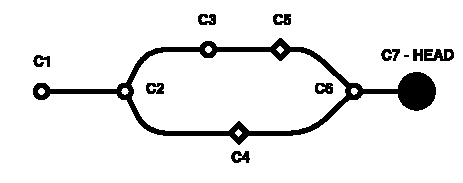
\includegraphics[width=0.5\textwidth]{cache.pdf}
    \caption{Example representation of commits history, with fix commits illustrated in a diamond shape}
    \label{fig:cache}
  \end{center}
\end{figure}


\subsection{Data Preparation}

This step is the simplest. The only task is to convert the raw JSON structure, focused on the commit, to a JSON structure, focused on the component. 7
Iterating through each file at the "\code{raw}" folder and creating a new one with the same name in the "\code{json}" folder.

The data contained in this new file will be ready for being converted to CSV and to be used for modeling or prediction.

The following columns are prepared for each component:
%
\begin{itemize}
\item \_\_changed - Was it changed?
\item \_\_filename - Component name
\item \_lines - Number of lines
\item \_bytes - File size in bytes
\item \_mostChanged - Was it the most changed file in this commit?
\item \_mostChanged25 - Was this file in top 25\% of most changed files is this commit?
\item \_mostChanged50 - Was this file in top 50\% of most changed files is this commit?
\item \_mostChanged75 - Was this file in top 75\% of most changed files is this commit?
\item changes - Number of changes made in the past
\item changes:date-weighted - Sum of the result of the time-weighted function applied to each change
\item changes:size-weighted - Sum of the number of lines added and removed in each change
\item changes:date+size-weighted - Sum of the result of the time-weighted function applied to each change multiplied for the number of lines added and removed in it
\item authors - Number of authors that changed this file
\item authorChanges::{author} - Number of changes made in the past by a specific author. E.g. authorChanges::luc@apache.org
\item authorChanges:date-weighted:{author} - Sum of the result of the time-weighted function applied to each change made by a specific author. E.g. authorChanges:date-weighted::luc@apache.org
\item authorChanges:size-weighted:{author} - Sum of the number of lines added and removed in each change made by a specific author. E.g. authorChanges:size-weighted::luc@apache.org
\item authorChanges:date+size-weighted:{author} - Sum of the result of the time-weighted function applied to each change made by a specific author multiplied for the number of lines added and removed in it. E.g. authorChanges:date+size-weighted::luc@apache.org
\end{itemize}

Being $t$ the normalized timestamp of the change, where 0 is the timestamp of the first commit and 1 of the latest, and $W = 12$, the time-weighted function used was the following:
%
\begin{equation}
  %\sum_{i=0}^{n}%
  \frac {1} {1 + e^{(-12 \cdot t) + W}}
\end{equation}

In order to improve modeling results, we also created the columns "changes-others", "changes-others:date-weighted", "changes-others:size-weighted", "changes-others:date+size-weighted", 
"changes-fixes", "changes-fixes:date-weighted", "changes-fixes:size-weighted" and "changes-fixes:date+size-weighted" that are equal to the already existing columns starting with
"changes", but refer only to changes that were not fixes and changes that were fixes, respectively.

Plotting the results we noticed that the date influenced significantly the data related to changes, since older commits have less history behind. 
So for each, we added a normalized version by the commit.

\begin{figure}[ht]
  \begin{center}
    \leavevmode
    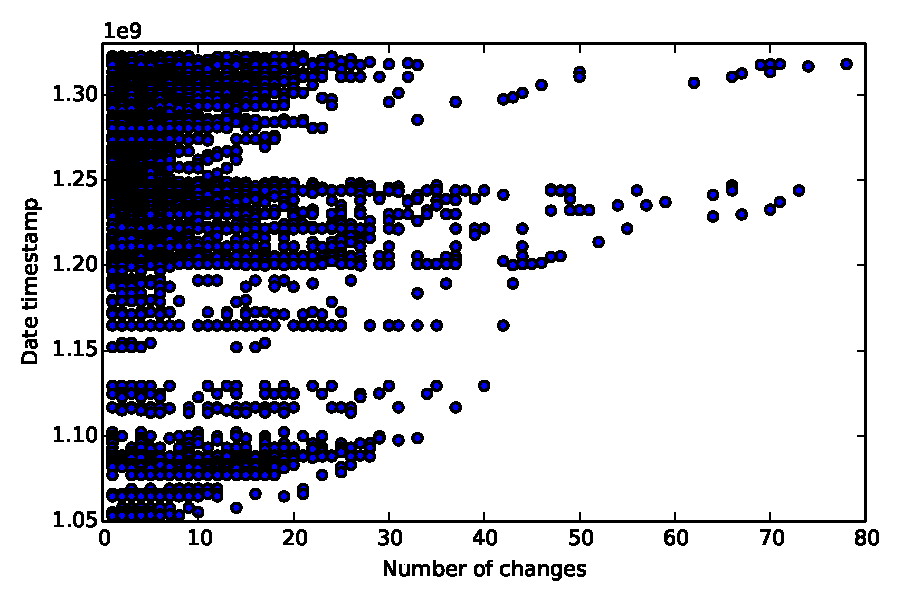
\includegraphics[width=0.75\textwidth]{date-changes_raw_math001.pdf}
    \caption{Example of the influence of the date on number of changes. (Project Math, Defect 1)}
    \label{fig:date-changes.raw}
  \end{center}
\end{figure}

\begin{figure}[ht]
  \begin{center}
    \leavevmode
    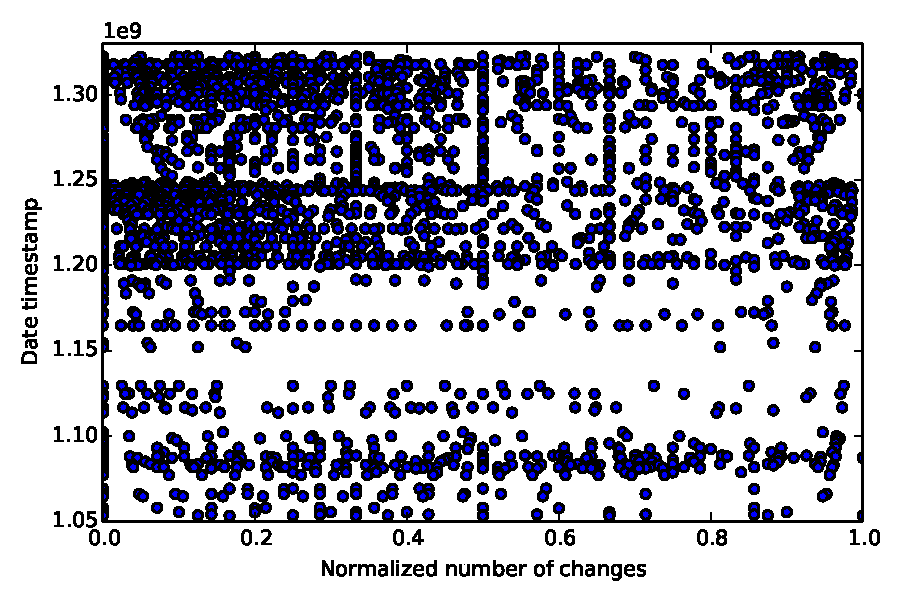
\includegraphics[width=0.75\textwidth]{date-changes_norm_math001.pdf}
    \caption{Example of the relation between the date on the normalized number of changes. (Project Math, Defect 1)}
    \label{fig:date-changes.norm}
  \end{center}
\end{figure}

\begin{lstlisting}
[
  {
    "__changed": true,
    "__date": 1364521362,
    "__filename": "src/main/java/org/apache/commons/math3/distribution/fitting/MultivariateNormalMixtureExpectationMaximization.java",
    "_lines": 441,
    "_bytes": 18211,
    "_mostChanged": false,
    "_mostChanged25": true,
    "_mostChanged50": true,
    "_mostChanged75": true,
    "changes:raw": 3,
    "changes:normalized": 0.2857142857142857,
    "changes-fixes:raw": 0,
    "changes-fixes:normalized": 0,
    "changes-others:raw": 3,
    "changes-others:normalized": 0.3333333333333333,
    "changes:date-weighted:raw": 2.979453,
    "changes:date-weighted:normalized": 0.290809968305134,
    "changes:size-weighted:raw": 481,
    "changes:size-weighted:normalized": 0.4746494066882416,
    "changes:date+size-weighted:raw": 477.701982,
    "changes:date+size-weighted:normalized": 0.4831911672918317,
    "changes-fixes:date-weighted:raw": 0,
    "changes-fixes:date-weighted:normalized": 0,
    "changes-fixes:size-weighted:raw": 0,
    "changes-fixes:size-weighted:normalized": 0,
    "changes-fixes:date+size-weighted:raw": 0,
    "changes-fixes:date+size-weighted:normalized": 0,
    "changes-others:date-weighted:raw": 2.979453,
    "changes-others:date-weighted:normalized": 0.3394176672358086,
    "changes-others:size-weighted:raw": 481,
    "changes-others:size-weighted:normalized": 0.4845814977973568,
    "changes-others:date+size-weighted:raw": 477.701982,
    "changes-others:date+size-weighted:normalized": 0.49340824785460163,
    "authors:raw": 3,
    "authors:normalized": 0.6666666666666666,
    "authorChanges::luc@apache.org:raw": 1,
    "authorChanges::luc@apache.org:normalized": 0,
    ...
    "authorChanges:date-weighted::luc@apache.org:raw": 0.993164,
    "authorChanges:date-weighted::luc@apache.org:normalized": 0.00025474141229450394,
    "authorChanges:size-weighted::luc@apache.org:raw": 33,
    "authorChanges:size-weighted::luc@apache.org:normalized": 0.5454545454545454,
    "authorChanges:date+size-weighted::luc@apache.org:raw": 32.774417,
    "authorChanges:date+size-weighted::luc@apache.org:normalized": 0.5455704368440787,
    ...
  },
  ...
]
\end{lstlisting}


The data from the multiple fix commits is then combined in a file named "history.csv" and the data from the \emph{HEAD} commit is placed at "master.csv". 
These two files will be only files required to execute the next step.


\subsection{Modeling and Prediction}

For modeling and predicting \emph{Python 3} and \emph{scikit-learn} is used.
Random Forests, Decision Trees and Naive Bayes were tried, but the former achieved significantly better results as it is presented in the Experimental Results chapter \ref{chap:exp-results}.
Neural Networks were not used since the training set is normally small.

Before training the model, the training set is randomized and balanced, first to a ratio of 5 \emph{clean} component for each \emph{buggy} component 
and then SMOTE is used to create more \emph{buggy} component entries. In order to train the model a \emph{Stratified KFold} (4 folds) is used and run 10 times, 
generating 40 different models. Performance of these 40 models is measured according to the difference of the mean defect probability of buggy test data and clean test data. 
The 15 models with the highest difference are then used to predict the defect probability of each component in the current project state and a mean is calculated.

As referred before, the results are saved directly at the repository folder.

%!TEX root = ../thesis.tex
\chapter{Barinel Integration}\label{chap:barinel-integration}

\section*{}

One of the objetives is to improve Barinel results and for doing so integrations with the existing Barinel project were made.
Priors replacement and results modification were the approaches chosen.

\section{Priors Replacement}

Barinel by default uses $\frac{1}{1000}$ as the defect probability (prior) for all software components (\ref{eq:4.1}).
%
\begin{equation} \label{eq:4.1}
  \pr(d) = \prod_{j \in d} \frac{1}{1000} \cdot \prod_{j \notin d} (1 - \frac{1}{1000})
\end{equation}

With this integration the Barinel project is now capable of receiving specific priors for each component, reading it from a CSV file located at the root of project being analyzed, and attributing them to the corresponding probes (\ref{eq:4.2}).
%
\begin{equation} \label{eq:4.2}
  \pr(d) = \prod_{j \in d} p_j \cdot \prod_{j \notin d} (1 - p_j)
\end{equation}


Maximum Likehood Estimation (MLE) continues to be used in order to maximize the probability, by defining the best possible goodness values.

\section{Results Modification}

The second approach maintains the priors at $\frac{1}{1000}$ and directly modifies the final result calculated by Barinel ($Pr(d_j, obs, e)$) by multiplying it by $2$ if considered faulty.
%
\begin{equation} \label{eq:4.2}
  Pr'(d_j, obs, e) = Pr(d_j, obs, e) \cdot 
  \begin{cases}
    2   & \textrm{if} j is faulty \\
	1  	& \textrm{otherwise}
  \end{cases}
\end{equation}

% TODO: Change this

%!TEX root = ../thesis.tex
\chapter{Experimental Results} \label{chap:exp-results}

\section*{}

In order to reliably validate the defect probability prediction we used an existing database of faults, \emph{Defects4J}.
This database contains a list of commits with defects and their location from five different projects (JFreechart, Closure compiler, Apache commons-lang, Apache commons-math and Joda-Time).
Since compatibility with \emph{Barinel} and using \emph{Git} is required, only the last three projects were used, making a total of 184 commits.
%
\begin{table}[H]
	\centering
	\begin{tabular}{|l|l|l|}
	\hline
	\textbf{Project name} & \textbf{Shortname} & \textbf{Defects} \\ \hline
	Apache commons-lang   & Lang               & 59               \\ \hline
	Apache commons-math   & Math               & 101              \\ \hline
	Joda-Time             & Time               & 25               \\ \hline
	\end{tabular}
	\caption{Test Set}
	\label{test-set}
\end{table}

\section{Estimating Defect Probability}

First we must know the characteristics of each project in order to better interpret the results, so a table was made containing information about the first and last commit of each
project.
%
\begin{table}[H]
\centering
\begin{tabular}{|l|l|l|l|l|l|}
\hline
\textbf{Project} & \textbf{Defect} & \textbf{Files} & \textbf{Previous commits} & \textbf{Previous fix commits} & \textbf{Contributors} \\ \hline
Lang             & 1               & 108            & 3569                      & 366                           & 40                    \\ \hline
Lang             & 59              & 81             & 1533                      & 190                           & 25                    \\ \hline
Math             & 1               & 813            & 4877                      & 564                           & 28                    \\ \hline
Math             & 103             & 370            & 957                       & 66                            & 15                    \\ \hline
Time             & 1               & 162            & 1717                      & 234                           & 27                    \\ \hline
Time             & 26              & 733            & 1474                      & 195                           & 9                     \\ \hline
\end{tabular}
\caption{My caption}
\label{my-label}
\end{table}

Three different classification algorithms were tested: Support Vector Machines, Random Forests and AdaBoost.
Our preliminary tests showed that Random Forests is the algorithm that provides an higher accuracy, that using the normalized values didn't help and the best label to use for training is \code{_mostChanged}, so we will focus on this test case.

In order to better understand the results it's important, not only to verify the predicted defect probability for the faulty component, but to compare this to the other components.
Since we want the faulty component to be the one with the highest defect probability. For example, although the predicted defect probability for the 15th fault of the Math project was only $0.29$, only $14.39\%$ components have a value above.

% TODO: Add reference to image

\begin{figure}[h]
  \begin{center}
    \leavevmode
    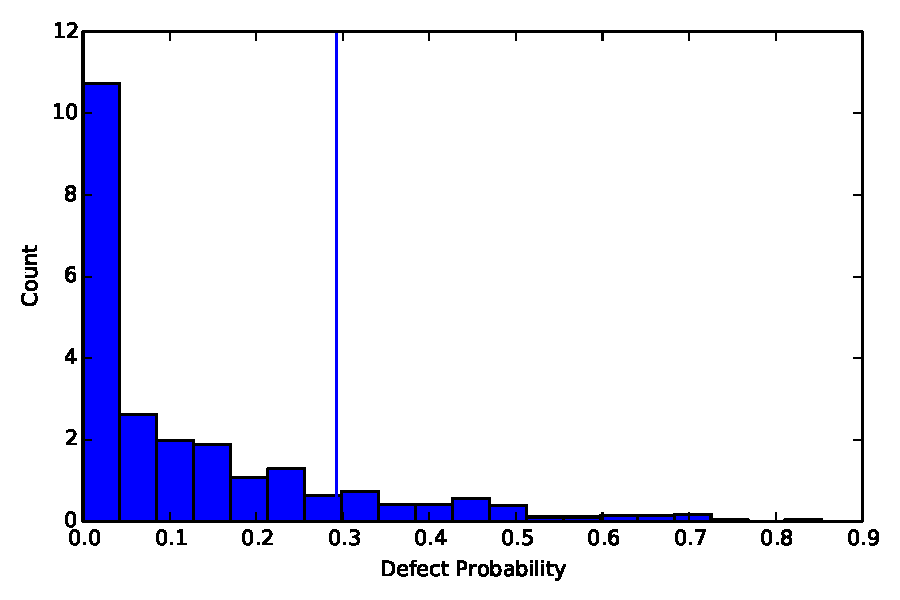
\includegraphics[width=0.65\textwidth]{dp-count_math015.pdf}
    \caption{Histogram of predicted defect probabilities for Project Math, Defect 15}
    \label{fig:dp-count_math015}
  \end{center}
\end{figure}

Analysing the data for the 188 defects, we concluded that the average percentage of components with higher defect probability than the faulty component is just $16.6\%$ and the median is $10.6\%$.

% TODO: Add reference to image

\begin{figure}[h]
  \begin{center}
    \leavevmode
    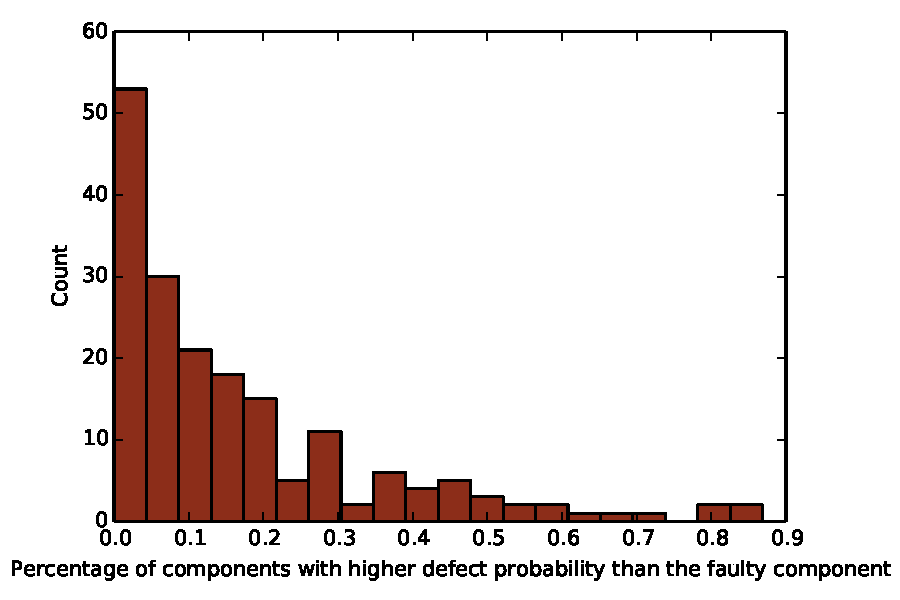
\includegraphics[width=0.65\textwidth]{faults-position.pdf}
    \caption{Histogram of the percentage of components with higher defect probability than the faulty component for all defects of all projects}
    \label{fig:dp-faults-position}
  \end{center}
\end{figure}

% GUIDELINES
% SVM vs Random Forests vs AdaBoost
% Relation between the value calculated for the wanted faulty classes vs others
% Example for one project (histogram of prediction. Vertical line - faulty) If more than one faulty use the higher predicted value
% Histogram for percentage positions of these faulty components


\section{Barinel Integration}

% Present the best possible results
% Present the results with 10% better or 10% worse
% Distribution of positions

Two types of integration with Barinel were tested so the results will be presented separately in the following two sub-chapters. However, in the interest of better understanding the results, an analysis of the results of the unmodified Barinel was made.

The unmodified Barinel analysis \ref{fig:fault-positions} showed that on $44.57\%$ of the 184 project states the faulty component already are on the first position and on $5.98\%$ it has associated a $0\%$ probability of being faulty. So, no improvements can be made on $50.55\%$ of the examples of the test set. It also showed that in $88.04\%$ of the results the component with the defect is above the 10th position. For the sake of this analysis, in case of draw, we consider the best position and won't consider on the graphics the cases where the associated probability is $0\%$.

\begin{figure}
  \begin{center}
    \leavevmode
    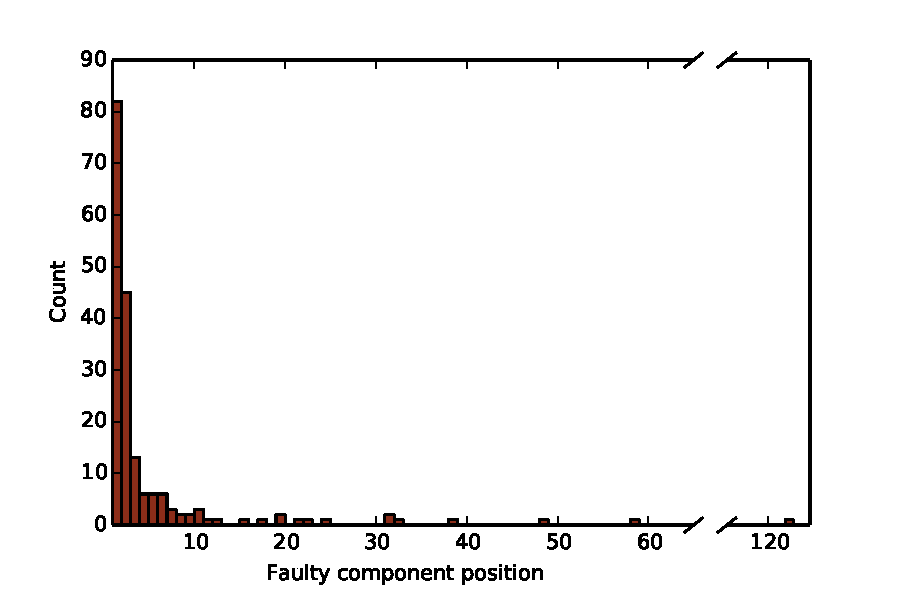
\includegraphics[width=0.65\textwidth]{unmodified-barinel_positions.pdf}
    \caption{Histogram of all the faulty component positions}
    \label{fig:fault-positions}
  \end{center}
\end{figure}


\subsection{Results Modification}

First, to be able to contextualize the results, the best and worst scenarios were tested. If the predicted defect faulty was 1 to all the faulty components and 0 for all the others, there would be an improve on 37 cases. If, for instance, the probabilities were totally wrong, it would worsen 54 cases.

Given the predicted defect probabilities is important to determine the best value to use as the minimum for a component to be considered possibly faulty. When considered possibly faulty, as explained in \ref{chap:chap4}, the Barinel fault probability is doubled. For each value from $0.5$ to $1$, at $0.05$ steps, the gain, loss and delta was calculated, as we can see in \ref{fig:results-modification}.

\begin{figure}
  \begin{center}
    \leavevmode
    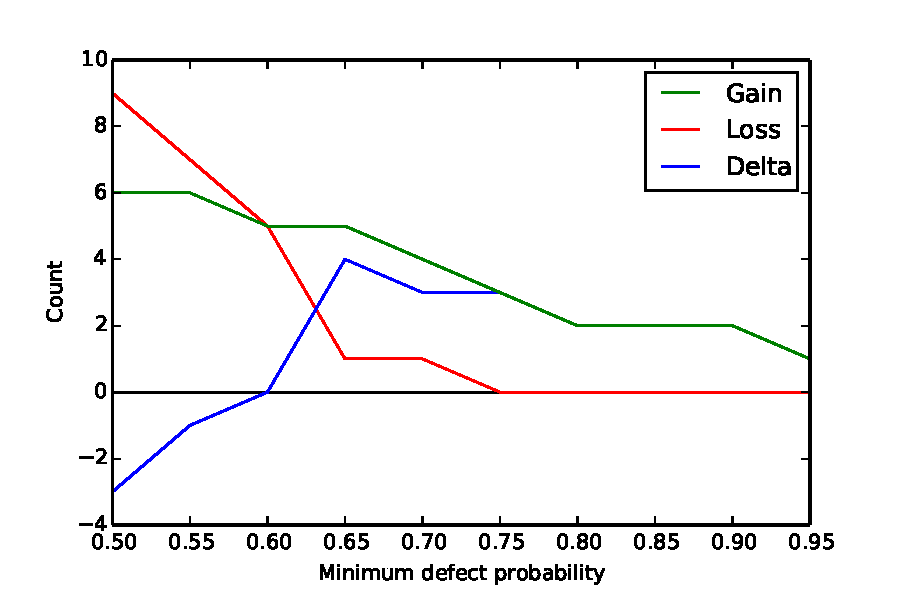
\includegraphics[width=0.65\textwidth]{barinel-integration-1.pdf}
    \caption{Results modification effect on Barinel results, by minimum defect probability}
    \label{fig:results-modification}
  \end{center}
\end{figure}


\subsection{Priors Replacement}

asdsad
% Chapter 6 - GUIDELINES

% (I think) it's cool at identifying hotspots
% It was able to do this being language agnostic and just by analysing the changes metadata
% commit message noise
% noise + unbalanced
% Improving Barinel it's hard
% Barinel results gains are small but reveal something
% To further improve Barinel results the defect probability prediction must be much more accurate
% Pq que há Outliers
% Zipf distribution
% -> Threats to validity
  % (internal) bugs no meu codigo
  % (construct) commit messages

% Conclusao

% It can and should be further worked
% Believe we can get better results by:
%  - Better handling noisy/unbalanced data
%  - Better identifying fixes
%  - Extracting static code data


%!TEX root = ../thesis.tex
\chapter{Discussion} \label{chap:discussion}

\section*{}

The experimental results acknowledged that extracting the component changes metadata is valuable by allowing to predict, with good precision and independently of the language, which files are more probable to have defects (Figure \ref{fig:dp-faults-position}).

\section{Estimating Defect Probability}

In figures \ref{fig:clean-dp-count} and \ref{fig:buggy-dp-count} we clearly see two distinct types of distributions. 
Probably clean components predicted defect probability tends to $0$, as intended, but the same can not be interpreted for the buggy components, whereas the distribution is more uniform. Preferably, the buggy components predicted defect probability distribution would tend more expressively to 1, being the reverse of figure \ref{fig:clean-dp-count}, but this may have been affected by the data imbalance and noise.

Since in each fix commit just a small percentage is changed and all the others are considered clean, extracted data is extremely unbalanced and the number of fault components in the training set is small. Using SMOTE improved the results, but the tendency to $0$ continues to be noticeable.

The assumption that all unmodified files are clean may also introduce noise in the data, by labeling faulty components as clean. This along with the uncertainty of the identification of fix commits by the commit message, that may lead to wrongly labeling clean components as faulty, may blur the difference between the two types and lower the prediction accuracy.

Besides, the faulty component may be defectuous just because of a recent change in a related component and since the data set does not contain any information about the components relations, it would be difficult for it to have a high predicted defect probability.

% Further more, one important aspect that can be observed on figure \ref{} and was verified by experimentation is that the model that allows to predict the faulty components now may not work in the future. The model must be trained with the most recent data, because the patterns that allow to identify to distinguish clean and fault component appear to change along with the project.

Yet, even with so much aspects that may affect our prediction accuracy, the figure \ref{fig:dp-faults-position} shows that, in fact, the faulty components tends to be classified as one of the components with the highest defect probability. Which is crucial to our goal of improving Barinel results.

\section{Barinel Integration}

Analysis of the unmodified Barinel, illustrated in \ref{fig:fault-positions}, showed how good the results are and the tenuous percentage of tests that can be improved by using our approach to modify Barinel results. $14.67\%$ in the best case scenario. While in the worst case scenario, $29\%$ of the tests would worsen.

Figure \ref{fig:results-modification} shows that when considering as faulty all the components with a predicted defect probability above $0.6$ the Barinel results improve, with little or no error. Examining for example the results for $0.65$ of minimum predicted probability, where the delta is higher, $13.5\%$ of the possible improvements occured and just one test worsened. Increasing the minimum diminishes both the number of improvements and errors, but starting at $0.75$ errors are completely eliminated.

Given this data, we can concluded with some confidence that components with a predicted defect probability above $0.65$ have in fact a high real defect probability.

\todo{The other barinel integration. + Flaky tests}

\section{Threats to Validity}

There are some threats to the validity of this research. The first is the fact that the Math project (101 tests of 184) appeared to have flaky tests, since with the exact same configuration Barinel, which is deterministic, reported some value changes. 

Using three open source Java projects, with 184 tests, may also not be sufficient to predict the application behaviour in other different projects

Being this research all about defect probabilities, we know that the application made to estimate the defect probability can also have defects and may somehow affect the predictions. Although the application was heavily tested and many results were manually checked for validity.

Last but not least, the data mining application is nondeterministic. It creates models every time and chooses the most accurate ones, in order to avoid being able to predict completely different results, but there will be most certainly differences as expected in a data mining project.



% Chapter 6 - GUIDELINES

% (I think) it's cool at identifying hotspots
% It was able to do this being language agnostic and just by analysing the changes metadata
% Difficulty to predict future based on the past
% commit message noise
% noise + unbalanced
% Improving Barinel it's hard
% Barinel results gains are small but reveal something
% To further improve Barinel results the defect probability prediction must be much more accurate
% Pq que há Outliers
% Zipf distribution
% -> Threats to validity
  % (internal) bugs no meu codigo
  % (construct) commit messages

% Conclusao

% It can and should be further worked
% Believe we can get better results by:
%  - Better handling noisy/unbalanced data
%  - Better identifying fixes
%  - Extracting static code data


%!TEX root = ../thesis.tex
\chapter{Conclusions and Further Work} \label{chap:conclusions}

\section*{}

We consider that building tools to help developers do a better job is crucial and have a huge positive impact on the global economy. 

By reviewing the available literature, it is possible to conclude that interest exists in bridging knowledge from the domain of Artificial Intelligence to Software Engineering.
This research aims to contribute to it.

\section{Goals contribution}

We set the goal at building a project that would be able to predict the component defect probability of any software project, written in any language, that uses \emph{Git}, with enough precision to improve Barinel results and achieved it. 

Even with experimental results showing that Barinel already classified the faulty component as one of the top 10 probably fauly components in $88.04\%$ of its results. 

So we can conclude that the project was successful and achieved the defined goals.


\section{Main Contributions}

Results confirm that it is possible to predict that a software component is faulty with $X\%$ of precision and $Y\%$ of recall, by using metadata information available at the Git repository and ignoring language-specific software metrics.

Research also revealed that using this information to calculate prior values improves Barinel results by $Z\%$.

Data mining application is open-source and can be already used with any \emph{Git} project to help identifying code hotspots. We consider that this capacity can help save time, by for example advising software developers doing code reviews to be more careful about specific files.

\section{Further Work}

Although the development and validation proved its concept and prediction capability, there is still room for development and future enhancements. Following are
some interesting ideas of future work.

\subsection{Improving fix commits identification}

In order to not depend on the usage of a bug tracker software, the fix commits identification is made by analysing the commit message. 

Since using this approach may introduce noise in the train set, which may lower the accuracy of the model, the bug tracker software information could be used when existing.

Other possible improvement is to enhance the regex used for the identification.

\subsection{Adding static code analysis features, when available}

The project showed that it is possible to not use static code analysis features to train a defect classifier. Nonetheless using those features would probably improve the model's accuracy. 

So, implementing such features for a set of languages and using them when possible could present interesting results.

\subsection{Improving machine learning model accuracy}

As stated in Chapter \ref{chap:discussion}, the train data set can be noisy and unbalanced. There are a wide range of different approaches to these problems and we have believe they could have a positive impact on the model's accuracy.

\subsection{Integrating with \emph{GitHub}}

Since the project showed to be able to predict that a software component has a defect with $X\%$ of precision and $Y\%$ of recall, it could be used to warn developers directly at \emph{Github} \footnote{\url{https://github.com}}.

Every time a pull request is created, the data mining application could analyze the project and if any changed file has a high defect probability or any changed files have their defect probability significantly increased a automatic comment would be made, alerting the submitter and the reviewers.

\subsection{Creating a different data structure to represent commit history tree}

Even with the performance improvements made through ignoring repeated tasks and caching the application is rather slow extracting the information from \emph{Git} and can benefit from more enhancements.

Project's performance can be enhanced, for example, by saving the commit history tree in a data structure that allows to more easily find past commits that changed a given file.

\subsection{Parallelization}

The extraction runs on \emph{node.js} so only one core is used at a time. Parallelization would improve application's performance and is possible, for example, using worker processes.

%% comment next 2 commands if numbered appendices are not used
% \appendix
% \chapter{Loren Ipsum} \label{ap1:loren}

Depois das conclusões e antes das referências bibliográficas,
apresenta-se neste anexo numerado o texto usado para preencher a
dissertação.

\section{O que é o \emph{Loren Ipsum}?}

\emph{\textbf{Lorem Ipsum}} is simply dummy text of the printing and
typesetting industry. Lorem Ipsum has been the industry's standard
dummy text ever since the 1500s, when an unknown printer took a galley
of type and scrambled it to make a type specimen book. It has survived
not only five centuries, but also the leap into electronic
typesetting, remaining essentially unchanged. It was popularised in
the 1960s with the release of Letraset sheets containing Lorem Ipsum
passages, and more recently with desktop publishing software like
Aldus PageMaker including versions of Lorem Ipsum~\citep{kn:Lip08}. 

\section{De onde Vem o Loren?}

Contrary to popular belief, Lorem Ipsum is not simply random text. It
has roots in a piece of classical Latin literature from 45 BC, making
it over 2000 years old. Richard McClintock, a Latin professor at
Hampden-Sydney College in Virginia, looked up one of the more obscure
Latin words, consectetur, from a Lorem Ipsum passage, and going
through the cites of the word in classical literature, discovered the
undoubtable source. Lorem Ipsum comes from sections 1.10.32 and
1.10.33 of ``de Finibus Bonorum et Malorum'' (The Extremes of Good and
Evil) by Cicero, written in 45 BC. This book is a treatise on the
theory of ethics, very popular during the Renaissance. The first line
of Lorem Ipsum, ``Lorem ipsum dolor sit amet\ldots'', comes from a line in
section 1.10.32.

The standard chunk of Lorem Ipsum used since the 1500s is reproduced
below for those interested. Sections 1.10.32 and 1.10.33 from ``de
Finibus Bonorum et Malorum'' by Cicero are also reproduced in their
exact original form, accompanied by English versions from the 1914
translation by H. Rackham.

\section{Porque se usa o Loren?}

It is a long established fact that a reader will be distracted by the
readable content of a page when looking at its layout. The point of
using Lorem Ipsum is that it has a more-or-less normal distribution of
letters, as opposed to using ``Content here, content here'', making it
look like readable English. Many desktop publishing packages and web
page editors now use Lorem Ipsum as their default model text, and a
search for ``lorem ipsum'' will uncover many web sites still in their
infancy. Various versions have evolved over the years, sometimes by
accident, sometimes on purpose (injected humour and the like). 

\section{Onde se Podem Encontrar Exemplos?}

There are many variations of passages of Lorem Ipsum available, but
the majority have suffered alteration in some form, by injected
humour, or randomised words which don't look even slightly
believable. If you are going to use a passage of Lorem Ipsum, you need
to be sure there isn't anything embarrassing hidden in the middle of
text. All the Lorem Ipsum generators on the Internet tend to repeat
predefined chunks as necessary, making this the first true generator
on the Internet. It uses a dictionary of over 200 Latin words,
combined with a handful of model sentence structures, to generate
Lorem Ipsum which looks reasonable. The generated Lorem Ipsum is
therefore always free from repetition, injected humour, or
non-characteristic words etc. 


%%----------------------------------------
%% Final materials
%%----------------------------------------

%% Bibliography
%% Comment the next command if BibTeX file not used
%% bibliography is in ``myrefs.bib''
\PrintBib{myrefs}

%% Index
%% Uncomment next command if index is required
%% don't forget to run ``makeindex thesis'' command
%\PrintIndex

\end{document}
